%%
% Please see https://bitbucket.org/rivanvx/beamer/wiki/Home for obtaining beamer.
%%
\documentclass{beamer}

\usetheme{Luebeck}
\usecolortheme{crane}
\setbeamertemplate{section in toc}[ball unnumbered]
\setbeamertemplate{subsection in toc}[ball unnumbered]

\usepackage[T1]{fontenc}
\usepackage{beramono}
\usepackage{graphicx}
\usepackage{hyperref}
\usepackage{pifont}
\usepackage{listings}
\usepackage{xcolor}
\usepackage{multicol}


%\definecolor{darkgreen}{rgb}{0.,0.6,0.}

\newcounter{questionizeIndex}

\newenvironment{questionize}[1][0]{%
    \setbeamercovered{invisible}%
    \setcounter{questionizeIndex}{#1}%
    \begin{itemize}%
}{ %
    \end{itemize}%
}

\newcommand{\question}[2]{%
    % #1: question
    % #2: answer (replaces question)
    \stepcounter{questionizeIndex}%
    \item<\value{questionizeIndex}->%
    \only<\value{questionizeIndex}>{#1}%
    \stepcounter{questionizeIndex}%
    \only<\value{questionizeIndex}->{#2}%
}

\newcommand{\lquestion}[4]{%
    % #1: question label
    % #2: question
    % #3: answer label
    % #4: answer (replaces question)
    \stepcounter{questionizeIndex}%
    \item[\only<\value{questionizeIndex}->{\alt<\value{questionizeIndex}>{#1}{#3}}]<\value{questionizeIndex}->%
    \only<\value{questionizeIndex}>{#2}%
    \stepcounter{questionizeIndex}%
    \only<\value{questionizeIndex}->{#4}%
}

\newcommand{\cquestion}[2]{\question{#2}{\color{#1}{#2}}}

\newcommand{\ctrue}[1]{\cquestion{darkgreen}{#1}}
\newcommand{\cfalse}[1]{\cquestion{red}{#1}}

\newcommand{\ltrue}[1]{\lquestion{\textbf{?}}{#1}{$\checkmark$}{#1}}
\newcommand{\lfalse}[1]{\lquestion{\textbf{?}}{#1}{$\times$}{#1}}

\lstset{
    basicstyle=\footnotesize\ttfamily,
    breaklines=true
}


\hypersetup{%
  colorlinks=true,% hyperlinks will be black
  pdfborderstyle={/S/U/W 1}% border style will be underline of width 1pt
}
\begin{document}

\title{MSiA490 SEC20/28\\ Text Analytics}
\subtitle{Lab 3 - Word2Vec and BERT}
\author{Timo Wang}
\institute{Northwestern University}
\date{October 1 2020}

\begin{frame}
    \titlepage
\end{frame}

\begin{frame}{Overview}
    \tableofcontents[hideallsubsections]
\end{frame}

\section{Discussions on Word2Vec and BERT}
\begin{frame}
    \frametitle{Discussions on Word2Vec and BERT}
    \begin{block}{Question1 }
        How is a Skip-gram model trained? What is its training objective? 
    How is BERT trained? What are its training objectives?
    \end{block}
\end{frame}

\begin{frame}
    \frametitle{Discussions on Word2Vec and BERT}
    \begin{block}{Question 1}
        How is the Skip-gram model trained? What is its training objective? 
    How is BERT trained? What are its training objectives?
    \end{block}
    \begin{block}{Notes 1}
        \begin{itemize}
            \item The training objective of the Skip-gram model is to maximize the average log probability of the context words.
            \item The training of BERT has two stages: pretraining and fine-tuning. The pretraining stage involves guessing the correct masked out word and predicting if the second sentence follows the first one.
        \end{itemize}
    \end{block}
\end{frame}

\begin{frame}
    \frametitle{Discussions on Word2Vec and BERT}
    \begin{block}{Question 2}
        What makes BERT different from Word2Vec models?
    \end{block}
\end{frame}

\begin{frame}
    \frametitle{Discussions on Word2Vec and BERT}
    \begin{block}{Question 2}
        What are some differences between BERT and Word2Vec?
    \end{block}
    
    \begin{block}{Notes 2}
        \begin{itemize}
            \item Word2Vec vector provides a vector for each token/word that encodes the meaning of that token/word. 
            \item BERT provides contextual word representations that encode different meanings under different context.
        \end{itemize}
    \end{block}
\end{frame}

\begin{frame}
    \frametitle{Discussions on Word2Vec and BERT}
    \begin{figure}
        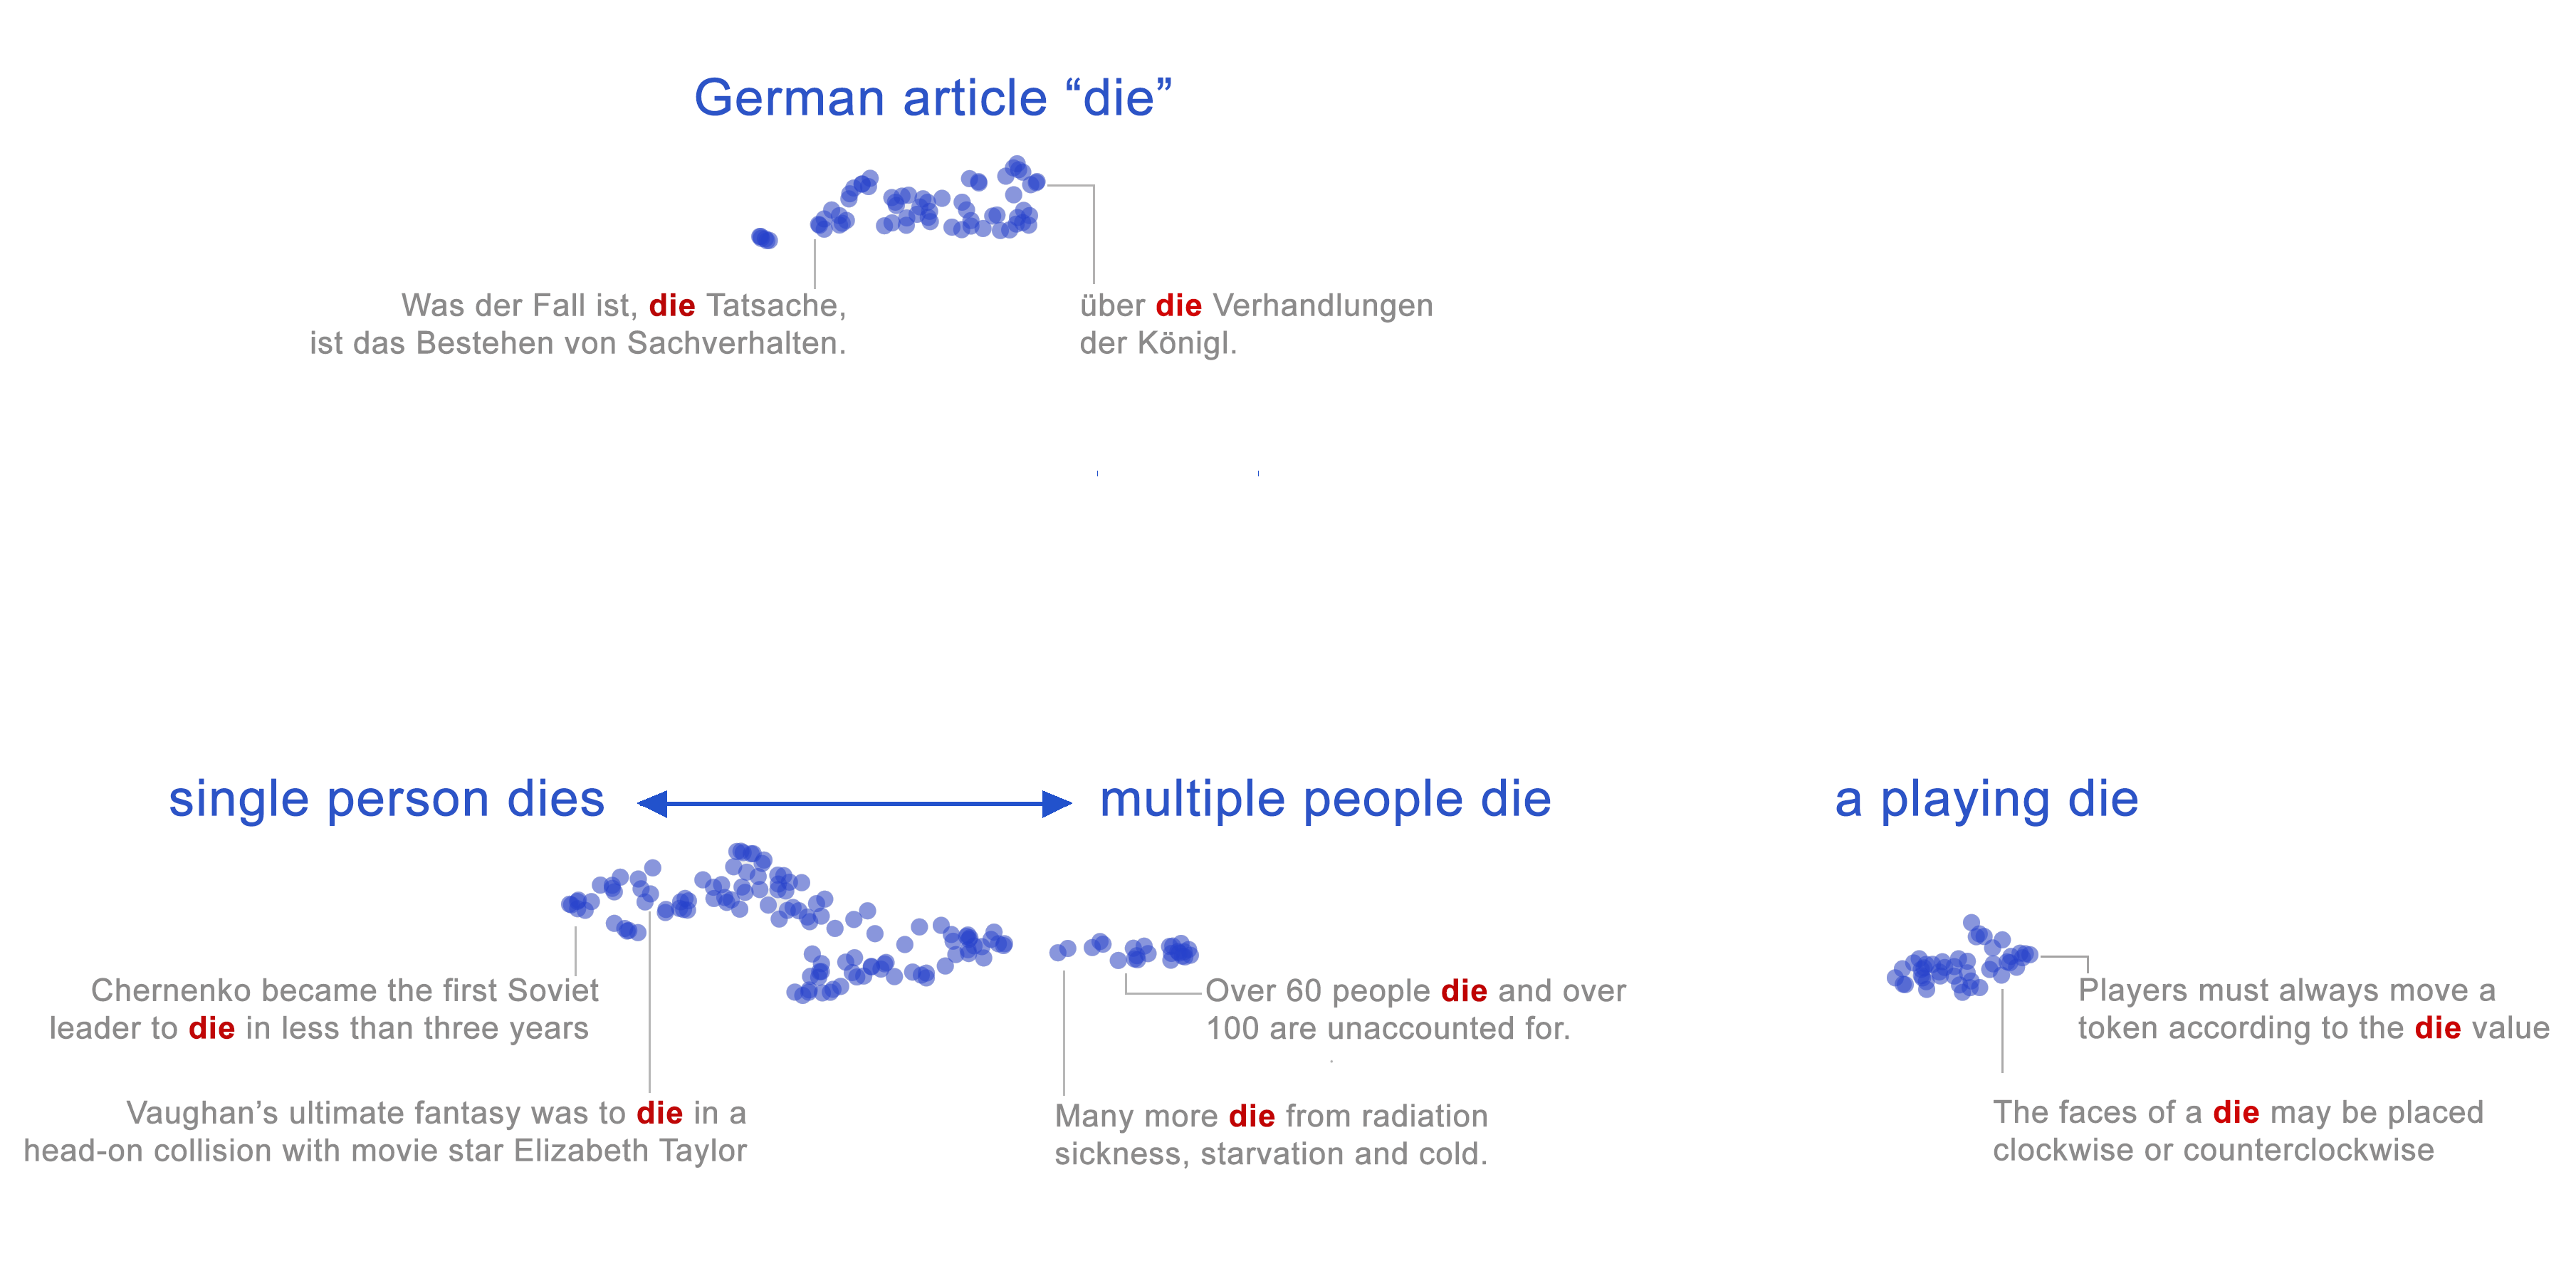
\includegraphics[scale=0.08]{visualize-bert}
        \caption{\footnotesize Embeddings for the word ``die'' in different contexts.\footnote{\tiny ``Visualizing and Measuring the Geometry of BERT''.\\ Coenen et al.}}
    \end{figure}
\end{frame}

\begin{frame}
    \frametitle{Discussions on Word2Vec and BERT}
    \begin{block}{Question 3}
        What are the advantages of pre-training for BERT? 
    \end{block}
\end{frame}

\begin{frame}
    \frametitle{Discussions on Word2Vec and BERT}
    \begin{block}{Question 3}
        What are the advantages of pre-training for BERT? 
    \end{block}
    
    \begin{block}{Notes}
        Pretraining BERT provides us with a generalized \textbf{language model} that can be used later for a variety of natural language processing tasks. The amount of training data required for those down streaming tasks does not need to be huge as the pre-trained model contains significant information on the language itself. 
    \end{block}
\end{frame}

\begin{frame}
    \frametitle{Discussions on Word2Vec and BERT}
    \begin{block}{Question 4}
        What are some down streaming tasks we can perform by fine-tuning BERT? 
    \end{block}
\end{frame}

\begin{frame}
    \frametitle{Discussions on Word2Vec and BERT}
    \begin{block}{Question 4}
        What are some down streaming tasks we can perform by fine-tuning BERT? 
    \end{block}
    
    \begin{block}{Notes}
        \begin{itemize}
            \item Single-sentence classification tasks
            \item Single-sentence tagging tasks
            \item Question answering tasks
        \end{itemize}
    \end{block}
\end{frame}

%\begin{frame}
%    \frametitle{Discussions on Word2Vec and BERT}
%    \framesubtitle{Word2Vec questions}
%    What is the problem with the original Skip-gram model?  How is it solved?  (Conceptual discussion is enough.)
%\end{frame}
%
%\begin{frame}
%    \frametitle{Discussions on Word2Vec and BERT}
%    \framesubtitle{Word2Vec questions}
%    What problem are hierarchical softmax/negative sampling trying to solve?
%\end{frame}

%\begin{frame}
%    \frametitle{Discussions on Word2Vec and BERT}
%    \framesubtitle{Word2Vec questions}
%    
%    What problem does subsampling of frequent words solve? 
%\end{frame}

\section{Using BERT}
\subsection{Hugging Face's Transformers}
\begin{frame}[containsverbatim]
    \frametitle{Using Bert}
    \framesubtitle{Hugging Face's Transformers}
    \begin{block}{Install}
        pip install transformers    
    \end{block}
    \begin{block}{Example usage}
    \begin{lstlisting}
> from transformers import BertTokenizer, BertModel

> tokenizer = BertTokenizer.from_pretrained("bert-base-uncased")
> model = BertModel.from_pretrained("bert-base-uncased")
> inputs = tokenizer("Hello world!", return_tensors="pt")
> outputs = model(**inputs)    
    \end{lstlisting}
    \end{block}


\end{frame}

\subsection{bert-as-service}
\begin{frame}
    \frametitle{Using Bert}
    \framesubtitle{Other options/resources}
    \begin{itemize}
        \item An alternative -- bert-as-service: \href{https://github.com/hanxiao/bert-as-service}{https://github.com/hanxiao/bert-as-service}
        \item A potentially outdated but still good tutorial on Hugging Face's Transformers: \href{https://mccormickml.com/2019/05/14/BERT-word-embeddings-tutorial/}{https://mccormickml.com/2019/05/14/BERT-word-embeddings-tutorial/} 
    \end{itemize}
\end{frame}

\section{Quiz}
\subsection{Task 1}
\begin{frame}
    \frametitle{Quiz}
    \framesubtitle{Task 1}
    Which of the following can be somehow realized with BERT but \textbf{not} with Word2Vec?
    \begin{enumerate}
        \item[A] Computing vectorized sentence representations
        \item[B] Computing vectorized word representations
        \item[C] Computing contextualized word representations
        \item[D] All of the above
    \end{enumerate}
\end{frame}

\subsection{Task 2}
\begin{frame}
    \frametitle{Quiz}
    \framesubtitle{Task 2}
    Which of the following is part of the pretraining stage for BERT?
    \begin{enumerate}
        \item[A] Single-sentence tagging
        \item[B] Masked-out word prediction
        \item[C] Next sentence prediction
        \item[D] A and B
        \item[E] B and C
        \item[F] A, B and C
    \end{enumerate}
\end{frame}
%
%\subsection{Task 3}
%\begin{frame}
%    \frametitle{Quiz}
%    \framesubtitle{Task 3}
%\end{frame}

%\section{Thoughts \& feedbacks}
%\begin{frame}
%    \frametitle{Thoughts \& feedbacks}
%    
%\end{frame}


\end{document}
